\item
Group I lists a set of four transfer functions. Group II gives a list of possible step responses $y(t)$. Match the step responses with the corresponding transfer functions.

\textbf{Group I}

\begin{tabular}{llll}
  $P = \frac{25}{s^2 + 25 }$ &
  $Q = \frac{36}{s^2 + 20s + 36}$ &
  $R = \frac{36}{s^2 + 12s + 36 }$ &
  $S = \frac{49}{s^2 + 7s + 49}$
\end{tabular}

\textbf{Group II}
\begin{figure}[H]\centering
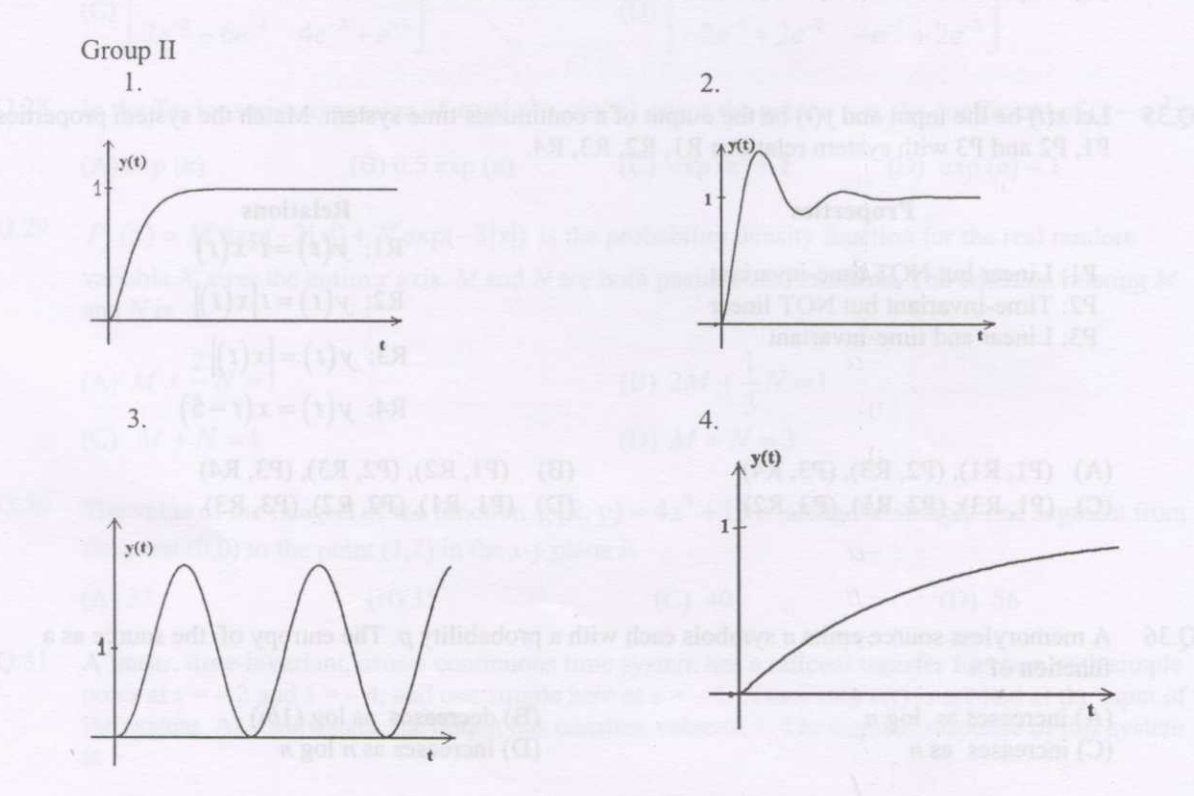
\includegraphics[width=0.9\columnwidth]{figs/2008/EC/q38.png}
\caption{Options}
\label{fig:q38}
\end{figure}
 
\hfill (EC 2025)
\begin{multicols}{2}
\begin{enumerate}
  \item P-3, Q-1, R-4, S-2
  \item P-3, Q-2, R-4, S-1
  \item P-2, Q-1, R-4, S-3
  \item P-3, Q-4, R-1, S-2
\end{enumerate}
\end{multicols}

\item A certain system has transfer function $G(s) = \frac{s+8}{s^2 + a s - 4},$ where $a$ is a parameter. Consider the standard negative unity feedback configuration.

\begin{figure}[H]\centering
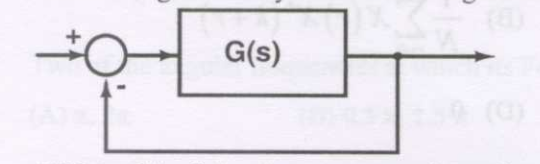
\includegraphics[width=0.5\columnwidth]{figs/2008/EC/q39.png}
\caption{Circuit}
\label{fig:q39}
\end{figure}

Which of the following statements is true?
 
\hfill (EC 2025)
\begin{enumerate}
  \item The closed loop system is never stable for any value of $a$.
  \item For some positive values of $a$, the closed loop system is stable, but not for all positive values.
  \item For all positive values of $a$, the closed loop system is stable.
  \item The closed loop system is stable for all values of $a$, both positive and negative.
\end{enumerate}
\newpage
\item A signal flow graph of a system is given below.

\begin{figure}[H]\centering
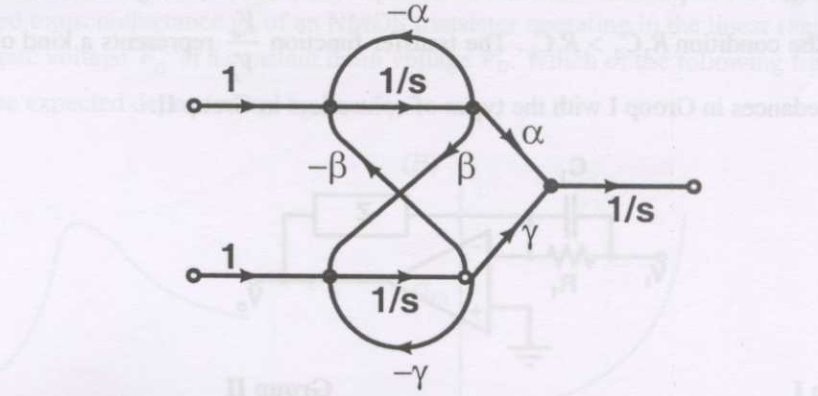
\includegraphics[width=0.5\columnwidth]{figs/2008/EC/q40.png}
\caption{Graph}
\label{fig:q40}
\end{figure}


The set of equations that correspond to this signal flow graph is
 
\hfill (EC 2025)
\begin{enumerate}
  \item $\frac{d}{dt}
    \myvec {
      x_1 \\ x_2 \\ x_3
    }
    =
    \myvec {
      \beta & -\gamma & 0 \\
      \gamma & \alpha & 0 \\
      -\alpha & -\beta & 0
    }
    \myvec {
      x_1 \\ x_2 \\ x_3
    }
    +
    \myvec {
      1 & 0 \\
      0 & 1 \\
      0 & 0
    }
    \myvec {
      u_1 \\ u_2
    }
   $
  \item $\frac{d}{dt}
    \myvec {
      x_1 \\ x_2 \\ x_3
    }
    =
    \myvec {
      0 & \alpha & -\gamma \\
      -\gamma & 0 & \beta \\
      \alpha & \beta & 0
    }
    \myvec {
      x_1 \\ x_2 \\ x_3
    }
    +
    \myvec {
      1 & 0 \\
      0 & 1 \\
      0 & 0
    }
    \myvec {
      u_1 \\ u_2
    }
   $
  \item $\frac{d}{dt}
    \myvec {
      x_1 \\ x_2 \\ x_3
    }
    =
    \myvec {
      -\gamma & 0 & \beta \\
      \alpha & \gamma & 0 \\
      -\beta & 0 & -\alpha
    }
    \myvec {
      x_1 \\ x_2 \\ x_3
    }
    +
    \myvec {
      1 & 0 \\
      0 & 1 \\
      0 & 0
    }
    \myvec {
      u_1 \\ u_2
    }
   $
  \item $\frac{d}{dt}
    \myvec {
      x_1 \\ x_2 \\ x_3
    }
    =
    \myvec {
      -\gamma & 0 & \beta \\
      0 & \alpha & 0 \\
      -\beta & 0 & -\alpha
    }
    \myvec {
      x_1 \\ x_2 \\ x_3
    }
    +
    \myvec {
      1 & 0 \\
      0 & 1 \\
      0 & 0
    }
    \myvec {
      u_1 \\ u_2
    }
   $
\end{enumerate}

\item The number of open right half plane poles of $G(s) = \frac{10}{s^3 + 2s^4 + 3s^3 + 6s^2 + 5s + 3}$ is
 
\hfill (EC 2025)
\begin{multicols}{4}
\begin{enumerate}
  \item 0
  \item 1
  \item 2
  \item 3
\end{enumerate}
\end{multicols}

\item The magnitude of frequency response of an underdamped second order system is 5 at 0 rad/sec and peaks to $\frac{10}{\sqrt{3}}$ at $5 \sqrt{2}$ rad/sec. The transfer function of the system is
 
\hfill (EC 2025)
\begin{multicols}{4}
\begin{enumerate}
  \item $\frac{500}{s^2 + 10s + 100}$
  \item $\frac{375}{s^2 + 5s + 75}$
  \item $\frac{720}{s^2 + 12s + 144}$
  \item $\frac{1125}{s^2 + 25s + 225}$
\end{enumerate}
\end{multicols}

\item
Group I gives two possible choices for the impedance $Z$ in the diagram. The circuit elements in $Z$ satisfy the condition $R_2C_2 > R_1C_1$. The transfer function $\frac{V_o}{V_i}$ represents a kind of controller. Match the impedances in Group I with the types of controllers in Group II.
\begin{figure}[H]\centering
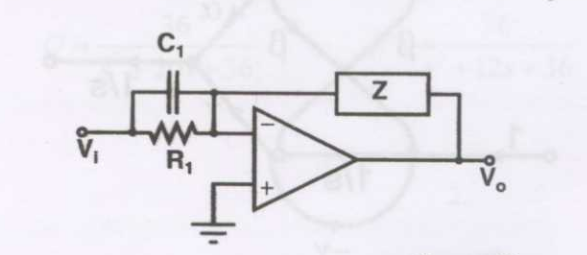
\includegraphics[width=0.8\columnwidth]{figs/2008/EC/q43a.png}
\caption{Circuit}
\label{fig:q43a}
\end{figure}
\textbf{Group I:}

\begin{figure}[H]\centering
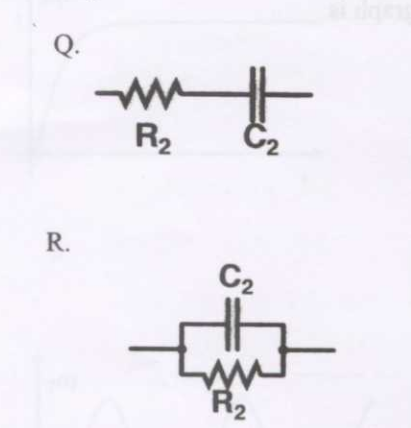
\includegraphics[width=0.4\columnwidth]{figs/2008/EC/q43b.png}
\caption{Group I}
\label{fig:q43b}
\end{figure}

\textbf{Group II:}

1. PID controller\hspace{1em}
2. Lead compensator\hspace{1em}
3. Lag compensator
 
\hfill (EC 2025)
\begin{multicols}{4}
\begin{enumerate}
  \item Q-1, R-2
  \item Q-1, R-3
  \item Q-2, R-3
  \item Q-3, R-2
\end{enumerate}
\end{multicols}

\item The OPAMP circuit shown above represents a
 
\hfill (EC 2025)
\begin{figure}[H]\centering
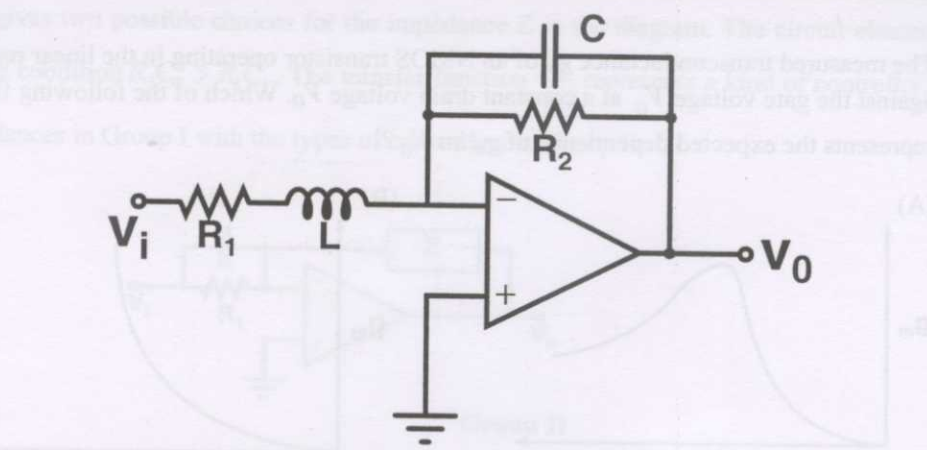
\includegraphics[width=0.5\columnwidth]{figs/2008/EC/q47.png}
\caption{Circuit}
\label{fig:q47}
\end{figure}

\begin{multicols}{2}
\begin{enumerate}
  \item high pass filter
  \item low pass filter
  \item band pass filter
  \item band reject filter
\end{enumerate}
\end{multicols}

\item Consider a Binary Symmetric Channel (BSC) with probability of error being $p$. To transmit a bit, say 1, we transmit a sequence of three 1s. The receiver will interpret the received sequence to represent 1 if at least two bits are 1. The probability that the transmitted bit will be received in error is
 
\hfill (EC 2025)
\begin{multicols}{2}
\begin{enumerate}
  \item $p^3 + 3p^2(1-p)$
  \item $p^3$
  \item $(1-p)^3$
  \item $p^3 + p^2(1-p)$
\end{enumerate}
\end{multicols}

\item Consider the frequency modulated signal $10\cos[2\pi \times 10^5 t + 5\sin(2\pi \times 1500 t) + 7.5\sin(2\pi \times 1000 t)]$ with carrier frequency of $10^5$ Hz. The modulation index is
 
\hfill (EC 2025)
\begin{multicols}{4}
\begin{enumerate}
  \item 12.5
  \item 10
  \item 7.5
  \item 5
\end{enumerate}
\end{multicols}

\item The signal $\cos \ohm_1 t + 0.5 \cos \ohm_f t \sin \ohm_t t$ is
 
\hfill (EC 2025)
\begin{multicols}{2}
\begin{enumerate}
  \item FM only
  \item AM only
  \item both AM and FM
  \item neither AM nor FM
\end{enumerate}
\end{multicols}

\end{enumerate}


\item A speech signal, band limited to 4 kHz and peak voltage varying between +5V and -5V, is sampled at the Nyquist rate. Each sample is quantized and represented by 8 bits.

\begin{enumerate}
\begin{enumerate}
\setcounter{enumi}{70}

\item If the bits 0 and 1 are transmitted using bipolar pulses, the minimum bandwidth required for distortion free transmission is
 
\hfill (EC 2025)
\begin{multicols}{4}
\begin{enumerate}
  \item 64 kHz
  \item 32 kHz
  \item 8 kHz
  \item 4 kHz
\end{enumerate}
\end{multicols}

\item Assuming the signal to be uniformly distributed between its peak to peak value, the signal to noise ratio at the quantizer output is
 
\hfill (EC 2025)
\begin{multicols}{4}
\begin{enumerate}
  \item 16 dB
  \item 32 dB
  \item 48 dB
  \item 64 dB
\end{enumerate}
\end{multicols}

\item The number of quantization levels required to reduce the quantization noise by a factor of 4 would be
 
\hfill (EC 2025)
\begin{multicols}{4}
\begin{enumerate}
  \item 1024
  \item 512
  \item 256
  \item 64
\end{enumerate}
\end{multicols}
\end{enumerate}
\item The following series RLC circuit with zero initial conditions is excited by a unit impulse function $\delta(t)$.
 
\begin{figure}[H]\centering
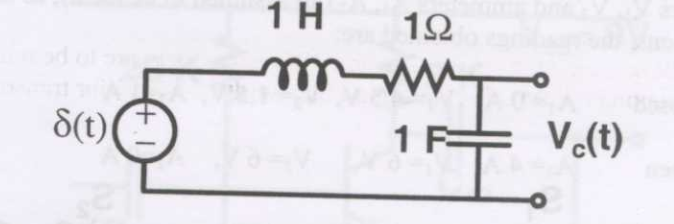
\includegraphics[width=0.6\columnwidth]{figs/2008/EC/q7475.png}
\caption{Circuit}
\label{fig:q7475}
\end{figure}

\begin{enumerate}
\setcounter{enumi}{73}

\item For $t>0$, the output voltage $V_c(t)$ is
 
\hfill (EC 2025)
\begin{multicols}{2}
\begin{enumerate}
  \item $\frac{2}{\sqrt{3}}\left(e^{-\frac{1}{2}t} - e^{-\frac{\sqrt{3}}{2}t}\right)$
  \item $\frac{2}{\sqrt{3}} t e^{-\frac{1}{2} t}$
  \item $\frac{2}{\sqrt{3}} e^{-\frac{1}{2} t} \cos\left( \frac{\sqrt{3}}{2} t \right)$
  \item $\frac{2}{\sqrt{3}} e^{-\frac{1}{2} t} \sin\left( \frac{\sqrt{3}}{2} t \right)$
\end{enumerate}
\end{multicols}

\item For $t>0$, the voltage across the resistor is
 
\hfill (EC 2025)
\begin{multicols}{2}
\begin{enumerate}
  \item $\frac{1}{\sqrt{3}} \left( e^{-\frac{\sqrt{3}}{2} t} - e^{-\frac{1}{2} t} \right)$
  \item $e^{-\frac{1}{2} t} \left[ \cos \left( \frac{\sqrt{3}}{2} t \right) - \frac{1}{\sqrt{3}} \sin \left( \frac{\sqrt{3}}{2} t \right) \right]$
  \item $\frac{2}{\sqrt{3}} e^{-\frac{1}{2} t} \sin \left( \frac{\sqrt{3}}{2} t \right)$
  \item $\frac{2}{\sqrt{3}} e^{-\frac{1}{2} t} \cos \left( \frac{\sqrt{3}}{2} t \right)$
\end{enumerate}
\end{multicols}

\end{enumerate}


\item In the following network, the switch is closed at $t=0$ and the sampling starts from $t=0$. The sampling frequency is $10$ Hz.
\begin{figure}[H]\centering
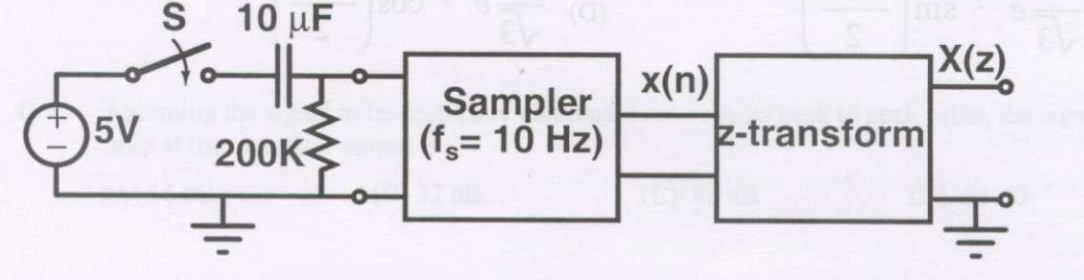
\includegraphics[width=0.6\columnwidth]{figs/2008/EC/q7879.png}
\caption{Circuit}
\label{fig:q7879}
\end{figure}

\begin{enumerate}

\item The samples $x(n)$ ($n=0,1,2,\ldots$) are given by
 
\hfill (EC 2025)
\begin{multicols}{4}
\begin{enumerate}
  \item $5 \left( 1 - e^{-0.05 n} \right)$
  \item $5 e^{-0.05 n}$
  \item $5 \left( 1 - e^{-5 n} \right)$
  \item $5 e^{-5 n}$
\end{enumerate}
\end{multicols}

\item The expression and the region of convergence of the $z$-transform of the sampled signal are
 
\hfill (EC 2025)
\begin{multicols}{2}
\begin{enumerate}
  \item $\frac{5z}{z-e^{5}};~ |z|<e^{5}$
  \item $\frac{5z}{z-e^{-0.05}};~ |z|<e^{-0.05}$
  \item $\frac{5z}{z-e^{-0.05}};~ |z|>e^{-0.05}$
  \item $\frac{5z}{z-e^{5}};~ |z|>e^{5}$
\end{enumerate}
\end{multicols}

\end{enumerate}

\item The impulse response $h(t)$ of a linear time-invariant continuous time system is given by
$h(t) = \exp(-2 t) u(t)$, where $u(t)$ denotes the unit step function.
\hfill (EC 2025)
\begin{enumerate}

\item The frequency response $H(\ohm)$ of this system in terms of angular frequency $\ohm$, is given by $H(\ohm) = $
 
\begin{multicols}{4}
\begin{enumerate}
  \item $\frac{1}{1 + j2\ohm}$
  \item $\frac{\sin \ohm}{\ohm}$
  \item $\frac{1}{2 + j\ohm}$
  \item $\frac{j\ohm}{2 + j\ohm}$
\end{enumerate}
\end{multicols}

\item The output of this system to the sinusoidal input $x(t) = 2 \cos (2t)$ for all time $t$ is
 
\begin{multicols}{2}
\begin{enumerate}
  \item $0$
  \item $2^{-0.25} \cos (2t - 0.125\pi)$
  \item $2^{-0.5} \cos (2t - 0.125\pi)$
  \item $2^{-0.5} \cos (2t - 0.25\pi)$
\end{enumerate}
\end{multicols}

\end{enumerate}


